\documentclass{article}
\usepackage{multirow}
\usepackage{longtable}
\usepackage{float}
\usepackage{parskip}
\usepackage[margin=0.75in]{geometry}
\usepackage{pgfplots}
\usepackage{graphicx}
\pgfplotsset{compat=1.18}
\title{Assignment 1}
\author{Garvit Shah [U21CS089]}
\date{January 2023}
\begin{document}
   \maketitle

   \section*{Hardware Details}
   \begin{itemize}
    \item Memory: 8 GB 1600 MHz DDR3
    \item Processor: 1.8 GHz Dual-Core Intel Core i5
  \end{itemize}

  \section*{Software Details}
  \begin{itemize}
   \item Apple clang version 14.0.0 clang-1400.0.29.202
   \item xcode-select version 2395.
  \end{itemize}

   \section{Insertion Sort}
   \subsection{Algorithm}
   \begin{enumerate}
    \item Create a file pointer and Open the File
    \item Read the number from the file and put it in an array.
    \item Start from second element and compare it with previous elements.
    \item If found appropriate position, insert at that position.
   \end{enumerate}
   
   \subsection{Observations}
   \begin{table}[h!] 
   \centering     
   \begin{tabular}{ | p{3cm} | p{3cm} | p{3cm} | }  
    \hline
    \multicolumn{3}{|c|}{Time Complexity for Insertion Sort} \\
    \hline
    File Name & No. of Entries & Average Case\\
    \hline 
    File-1 & 1024 & 0.003174 \\ 
    File-2 & 4096 & 0.048634 \\ 
    File-3 & 16384 & 0.777577 \\ 
    File-4 & 65536 & 12.446997 \\ 
    File-5 & 262144 & 199.183045 \\ 
    File-6 & 1048576 & 3187.061125 \\ 
    File-7 & 2097152 & 12748.334020 \\ 
    File-8 & 4194304 & 50993.515653 \\ 
    File-9 & 8883608 & 228757.176227 \\ 
    File-10 & 16777216 & 815898.409093 \\  [1ex]
    \hline
   \end{tabular}
   \caption{Time taken for Insertion Sort}
\end{table}
\newpage
\subsection{Graph}
\begin{center}
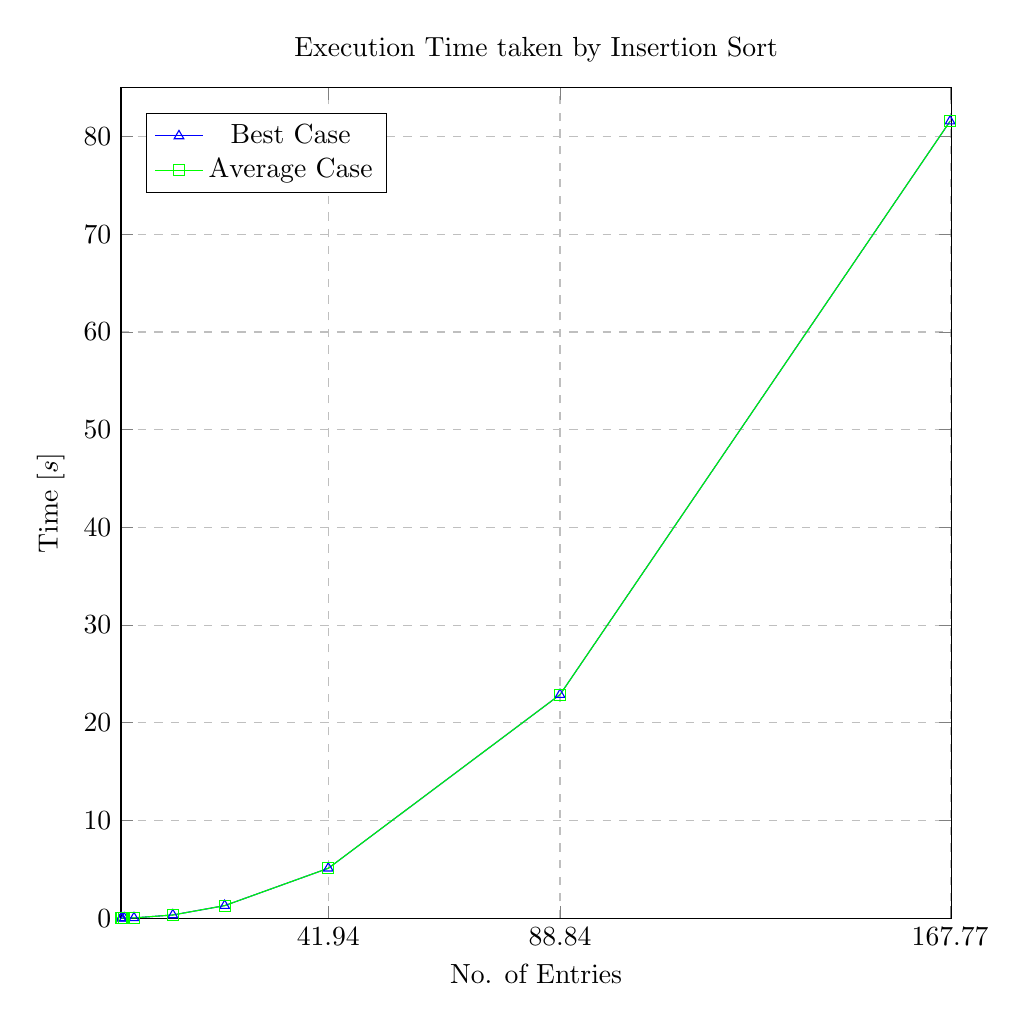
\begin{tikzpicture}
   \begin{axis}[
       title={Execution Time taken by Insertion Sort},
       xlabel={No. of Entries},
       ylabel={Time [\(s\)]},
       xmin=0, xmax=168,
       ymin=0, ymax=85,
       xtick={41.94304,88.83608,167.77216},
       ytick={},
       height = \textwidth,
       width = \textwidth,
       legend pos=north west,
       grid = both,
       grid style=dashed,
       legend entries = {Worst Case}
   ]
   \addplot[
       color=blue,
       mark=triangle,
       ]
       coordinates {
       (0.01024,0.0000003174)(0.04096,0.0000048634)(0.16384,0.0000777577)(0.65536,0.0012446997)(2.62144,0.0199183045)(10.48576,0.3187061125)(20.97152,1.2748334020)(41.94304,5.0993515653)(88.83608,22.8757176227)(167.77216,81.5898409093)
       };
    
    \addplot[
    color=green,
    mark=square,
    ]
    coordinates {
    (0.01024,0.0000003174)(0.04096,0.0000048634)(0.16384,0.0000777577)(0.65536,0.0012446997)(2.62144,0.0199183045)(10.48576,0.3187061125)(20.97152,1.2748334020)(41.94304,5.0993515653)(88.83608,22.8757176227)(167.77216,81.5898409093)
    }; 
    
    \legend{Best Case, Average Case}
   \end{axis}
   \end{tikzpicture}
\end{center}

\subsection{Conclusion}
The graph for the worst case is a quadratic. A quadratic curve implies that
the change in time taken is quadratically dependent on the change in the no. of elements in the file,
as the line is given by $y = 4ax^2$.
Therefore, it can be concluded that the time complexity for Insertion Sort is $O(n^2)$.
Theoretically also time complexity comes out to be $O(n^2)$. Thus the conclusion matches to the theoretical
value of the time complexity.

\textbf{Time Complexity = $\theta(n)$}
\end{document}